\documentclass{article}%
\usepackage[T1]{fontenc}%
\usepackage[utf8]{inputenc}%
\usepackage{lmodern}%
\usepackage{textcomp}%
\usepackage{lastpage}%
\usepackage{authblk}%
\usepackage{graphicx}%
%
\title{Upregulation of PIAS1 protects against sodium taurocholate{-}induced severe acute pancreatitis associated with acute lung injury}%
\author{Jill Gray}%
\affil{Department of Neurology, The Agnes Ginges Center for Human Neurogenetics, Hadassah University Hospital, Jerusalem, Israel}%
\date{01{-}01{-}2012}%
%
\begin{document}%
\normalsize%
\maketitle%
\section{Abstract}%
\label{sec:Abstract}%
The U.S. Food and Drug Administration said Friday that the products most closely linked to Salmonella enterica Type III were the same as those previously tested for the type of product used for Merck \& Co.'s melamine vaccine.\newline%
The researchers performed their analysis in the Science Translational Medicine Institute panel for experimental vaccines, which panelists heard a panelist from that company address specifically.\newline%
FDA scientists added a new variable to the review of the results, a factor that more than half of the panelists agreed could impact the expected failure rate for the vaccine, the FDA said.\newline%
The analysis began last May, and the FDA is expected to issue its conclusions in an upcoming regulatory order.\newline%
Whew! When the clock struck 11 p.m. Friday, I just got fired from my company of nearly 6 years.\newline%
I was jobless for five days and week. I was in the middle of one of the worst temp jobs in the history of science, and we still have the lunch box. Did I get my degree, or can I get out of here?\newline%
By the end of this government shutdown it might have been sooner.\newline%
This is the first time in 30 years FDA has been able to take action and stop a preventable disease outbreak from occurring because of failures to act responsibly on a voluntary basis.

%
\subsection{Image Analysis}%
\label{subsec:ImageAnalysis}%


\begin{figure}[h!]%
\centering%
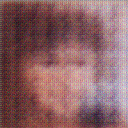
\includegraphics[width=150px]{500_fake_images/samples_5_99.png}%
\caption{A Black And White Photo Of A Black And White Cat}%
\end{figure}

%
\end{document}